\chapter{Planning}

This chapter is about how we planned our project. The purpose of this chapter is to explain how our team is organized, who we are, why we do this project and how do it.

\section{Overall project plan}

\subsection{Project name}
Formal and secure messaging on a mobile platform.

\subsection{Project sponsor}

The customer for this project is Thales Norway AS. Thales is a leading international electronics and systems group, focusing on defence, aerospace and security markets worldwide. The leading-edge technology in use at Thales offers capabilities unmatched in Europe for development and deployment of mission-critical information systems proven in the field. The group’s civil and military business areas develop in parallel and share a common base of technologies to serve a single objective: the security of people, property and nations.
\\
\\
After Thales’ 50 years of industrial activity in Norway it is now one of Norway’s largest industrial centres of expertise for mission-critical IT and telecommunications solutions and the principal supplies if military communication systems to the Norwegian Armed Forces. [1]

\subsection{Involved Parties}

In this project there are only three involved parties: a) the customer b) the project team and c) the advisor. The customer Thales, as described in the section above, was represented by Christian Tellefsen and Stig Bjørlykke. The project team consists of 6 students from the Department of Computer and Information Science (IDI) at the Norwegian University of Science and Technology (NTNU).The advisor was Mohsen Anvaari who was assigned to our team to guide and help us during the project period.

\subsection{Background for the project}

This project was given us as an assignment in the course TDT4290 Customer Driven Project. Since the society is constantly changing, the technology must follow the enormous changes we see today. Because of these changes Thales found that they needed an handheld android version of their now existing XOmail system. This new handheld system would help the users of XOmail so that they could also use it in the field and not only at the office. When able to use this mailing system not only in contact of a computer the regular working day of Thales customers would be a lot easier, especially since the primary customer is the norwegian military.

\subsection{Measurement of project effects}

Thales has proposed the following effects:
\begin{itemize}
\item{}Test user interface for message-based communication on a handheld device
\item{}Make a prototype that can give inspiration for further product development and be used as a demonstration internally and to customers
\end{itemize}

\newpage
\subsection{General terms}

\subsubsection{Technical Limitations}

\paragraph{Android}
Android is a quite new platform and none of us have been doing much programming in Android before starting on this project. So to learn how Android works and to find technical tools that Android supports is going to be a time consuming task. We will develop our project in Android version 2.2 with API level 8. 

\paragraph{Screen}
The mail client will be used on devices with relatively small touch screens, which means that the design must be carefully carried out to accommodate this requirement and be easy to use. The application must be designed as to scale to different screen resolutions. 

\subsubsection{Non-technical Limitations}

\paragraph{Language}
The entire project is to be delivered in English, so we all have to write in our second language. This causes that the time it takes to writes this document will be longer than if we could write in Norwegian.

\paragraph{Time}
We have a set timeframe on 13 weeks with a delivery deadline that can’t be changed. This gives us an set amount of time, and we probably won’t have the time to implement and do everything we want with the application, but only the necessary implementations so that when we are finished the application works the way it should. This specified timeframe gives us challenges when it comes to planning, and priorities of the different tasks.

\subsubsection{Tool Selection}

\paragraph{Git and GitHub}
Git is an extremely fast, efficient, distributed version control system ideal for the collaborative development of software and GitHub is the best way to collaborate with others. Fork, send pull requests and manage all your public and private git repositories. We use git to make it easy to share and work with the same source codes through this project.

\paragraph{Google Docs}
Google Docs is a free Web-based service that offers users the ability to create and edit documents online. Google docs lets us share documents easily and collaborate on the same document simultaneously.    

\paragraph{NetBeans IDE}
NetBeans IDE is an integrated development environment for developing with Java. It is written in Java and can run on both Windows and OS X. NetBeans IDE is one of the best IDEs and helps speed up the development process.

\paragraph{Apache Maven}
Maven is a build automation tool which is typically used with Java projects. It uses an XML file to describe the project, the project dependencies on other external modules and components, the build order, directories, and required plug-ins.  

\paragraph{JIRA with GreenHopper extension}
JIRA is and issue tracking system developed by Atlassian that is used for bug tracking, issue tracking and project management. Along with the GreenHopper extension it adds support for agile development.

\paragraph{LaTeX}
LaTeX is a document markup language and document preparation system for the TeX typesetting program. LaTeX was chosen because of the high quality of typesetting which TeX provides. 

\subsubsection{Organizational demands}
There are no organizational demands from Thales, but agreed that a Scrum based approach is good, as this gives a running product that can be commented on during the project. This is a pilot project and the specifications are not fully completed, so many revisions as we go are anticipated. 

\subsubsection{Resources}
We are a very diverse group which has its points in favour and against. We are all students that are working on a master degree in computer science, but the programming experience of each member varies. Two of the group members have programmed since they were about thirteen years old, while the rest started when they came to NTNU. All of us has at some point had a programming job, and are therefore used to working in teams. 

\newpage
Luckily, one might say, we all have different interests regarding what we would like to contribute with. It is a common understanding that we all have to take our part of the programming, documentation and the report work, but as one likes to do documentation, another the report work and one has much experience in set up of programming related tasks, all have gotten their main roles accordingly. 
\\
\\
The range of person gallery also gives a good group dynamic, making the group meetings efficient. By having a daily stand up where everyone shares what they have done, what they should do and what they need to get it done, we are able to get a common understanding of what needs to be done, and everyone get in sync.

\subsection{Duration}
The course staff has suggested a calculated 25 hour weeks for each student. This will give us a total of 1950 working hours since we are 6 students in our team, and that the project is distributed over 13 weeks.

\begin{itemize}
\item{}Project start: 21.08-2012
\item{}Project finish: 22.11-2012
\end{itemize}

\subsection{Schedule of results}

\subsection*{Milestones}
See table \ref{tab:milestones} at page \pageref{tab:milestones}
\begin{table}
\begin{tabular}{l|l}
Project start &  21.08.2012\\ \hline
Pre-delivery of project report & 14.10.2012\\ \hline
Final delivery of project report & 22.11.2012\\ \hline
Project presentation and demonstration & 22.11.2012
\end{tabular}
\caption{Milestones} \label{tab:milestones}
\end{table}

\subsection*{Sprints}
See table \ref{tab:sprints} at page \pageref{tab:sprints}
\begin{table}
\begin{tabular}{l|l}
Sprint 1 &  27.08.2012 - 16.09.2012\\ \hline
Sprint 2 & 17.09.2012 - 07.10.2012\\ \hline
Sprint 3 & 08.10.2012 - 28.10.2012\\ \hline
Sprint 4 & 29.10.2012 - 18.11.2012
\end{tabular}
\caption{Sprints} \label{tab:sprints}
\end{table}

\begin{figure}[htb]
\begin{center}
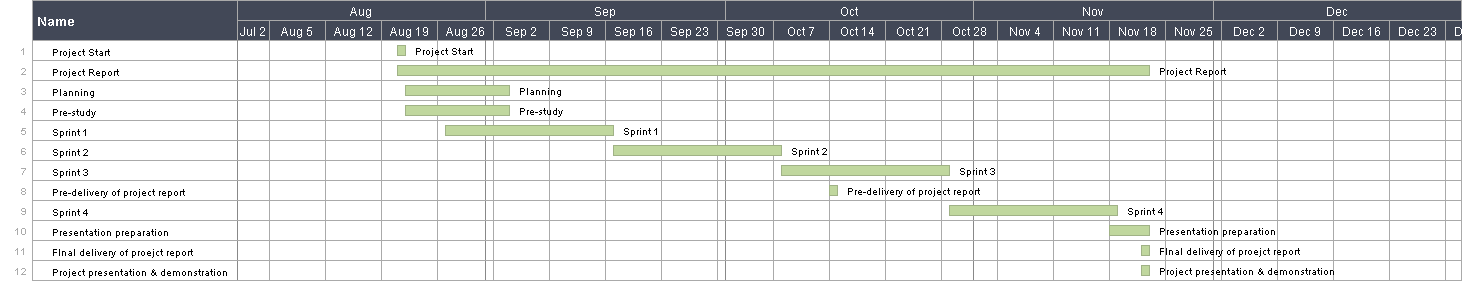
\includegraphics[width=\textwidth, height=2.5in]{foo}
\caption{Gantt-diagram for the entire project}
\end{center}
\end{figure}